%----------------------------------------------------------------
%
%  File    :  survey-animation.tex
%
%  Author  :  Fernando Pulido Ruiz, TU Graz, Austria
% 
%  Created :  01 Dec 2016
% 
%  Changed :  Changed :  04 Dec 2016
% 
%----------------------------------------------------------------


\chapter{Animation}

\label{chap:Animation}

{\em"Animation is defined as changing some property over time. On the other 
hand, motion is the act of moving or the process of being moved. . . .  To put 
it more simply, all motion is animation, but not all animation is 
motion."}\citep{head2016designing}

\section{Not Just Motion!} % (fold)
\label{sec:anime_motion}

In animation we change an object’s attribute(s) over time to achieve an 
objective. As stated by \citet{head2016designing}, animation is much more than 
adding movement to an object. Movement of an object can be described by a 
change of its 6 degrees of freedom, them being the coordinates in 3D space and 
the rotation around the 3D space axises. However an object has usually many 
more changeable attributes or properties. One could animate color changing and 
fading, invisibility through transparency, growth with scaling, focus with 
blurring, etc.

\section{Why Animation in Web UI?} % (fold)
\label{sec:anime_why}

While writing this survey, with so much animation theory, a hilarious idea was 
just coming up to mind. Have you ever stopped to think about why some people 
just seem to be more funny than others? And of course, this happens everyday. 
Just think about a good joke told by someone with no real humour. It is 
meaningless. Now, think about the same joke being told by a profesional 
comedian on TV telling jokes over the weekend. Way more funny, is it not? But 
the point is, why and how is this be possible?
It has lots to do with how they speak and how they move! As well of other minor 
factors. That, I am afraid, is the same as with animation. To have a better 
understanding of what factors are involved and how they can improve the user 
experience in UIs, we look deeper into it in this section with 
\citet{head2016designing} as the reference point.

Animation, be it in a cartoon, webpage, app or anywhere else, adds a new level 
of communication which can be hard to explain , but easy to feel. It creates a 
special connection between what the message is intended to be, and the 
receiver. It allows an additional cannel of invisible information to exist, and 
makes the viewer feel part of the process, and gets his attention grabbed in a 
practical way.

We always need to understand, where we are and where are we going to. Animation 
can helps us with this and even can improve the use of resources. Just think 
about when trying to navigate through a small screen. Having some animated 
window coming out when you put your mouse on, does not only save space (which 
is already a good enough reason to implement it), but makes the entire process 
of navigating easier and simpler. A user does not really want to think while 
navigating, and this can be fulfilled with animation. They can be guided, 
orientated or helped in going through a process just with animation, which will 
of course improve their user experience and make them feel more sure and 
comfortable about what they are doing, without thinking they are in a real 
puzzle and need to make big use of their brains.

Putting it all together, we can effectively ensure that a well planned 
animation will improve decision making, as it will guide the user through the 
entire process, allowing him to be more aware about the real process or task he 
or she is willing to achieve, and not about the real animation. Of course, this 
can be enforced by the fact that the user will feel listened and will probably 
trust more the site because of the animation being interactive, giving in some 
way feedback, making the user feel comfortable when its input is being taken 
into consideration.

Nowadays, it´s very common to access many sites through different devices. 
Just think about when trying to know any train timetable. You probably have the 
app in your Smartphone, but depending on where are you at the moment, you might 
just google it up and search it through their webpage. Having animation allows 
sites to connect context and media. A user will just find himself guided 
throught the process no matter where he is or what device is he using, because 
of being under some potential animation process. 

But, how do these animations grab people´s atention? There are over twelve 
basic principles, written by Disney, but two of them are like the foundation of 
animation, and the rest basically build up from them. Timing and spacing. 
Timing can be understood as the time length of an action to happen, let’s say 
the duration of it, while spacing could be explained as the speed changes 
during one of these actions in an animation. 
\citet{head2016designing} (Chapter 2, page 18) describes their impact with: 
{\em“Timing and spacing convey the mood, emotion, and reaction of an 
object.”}

\section{Aim For Invisible Animation} % (fold)
\label{sec:anime_invisible}

In animation, it is very common during the designing process to end up messing 
things up. As a general rule, as a designer, your one good way to show love to 
the user is actually not making his or her life harder accomplishing the task 
at hand. Certainly designers do not hold such ill intentions, but as said 
before, it is quite easy and happens very often just to have users unnecesarily 
waiting for an animation to finish or having a hard time finishing a task due 
to animation. It could be said that the perfect animation is the one which is 
not noticed. That´s not 100\% accurate, but a good idea in general. 

\vspace{5mm}

{\em“Good interface animations need to be flexible and always feel responsive 
to a user’s input even if the animation is currently 
animating.”}\citet{head2016designing} (Chapter 3, page 48)

\vspace{5mm}

Users need feedback to feel themselves listened and understood. Animation can 
be understood as a bridge which takes the user to a higher quality experience. 
If an animation doesn’t respect having the user happily informed with 
feedback, its experience quality will of course drop and so will the trust 
towards the UI. A user will never feel comfortable in a system which does not 
take into consideration its input. 

It is also important, that an animation should never be a show-off work. It 
should be always remembered, that in general, the user interacting with an 
animation, is probably willing to do or finish something. A UI user is not just 
laying there waiting for an animation to happen and look at it itself and enjoy 
it. That could be the aim of animators years ago where they were really telling 
stories and people were fascinted about it. But times changed, and now the 
timing requirements are no longer the same as in those days. Study and 
carefully think about the suitable timing for each animation, because a short 
amount of milliseconds can be the limit between failing or succeeding. Good 
timing is more an art than a science \citep{head2016designing}.

\section{Development of Animation} % (fold)
\label{sec:anime_dev}

There are lots of guidelines to help developers through the development of an 
animation, but what about some guidelines for the actual development itself? 
When coming up to a project, the animation issues are often discussed at the 
end of it. It is quite normal to just understand animation in a project as 
extra decoration, as something which is not mandatory, which will just make the 
whole running project look a little nicer. This should not be the way of 
proceeding, but it is the reality of many projects. Animation should be part of 
the design, due to the potential for a better user experience, like described 
in section \ref{sec:anime_why}. Just bare in mind that when the project is 
finished, it is usually too late to replan the design involving animation at 
its full potential, and this leads to many projects to just leave beside some 
good animation ideas.
Trying to makes things easier for the user (that is what animation is all 
about) at the end of a project, when everything is quited fixed, doesn´t sound 
like a good plan. Always start planning animation schemes in early stages! It 
is always better to have a pause after each step of the project design to talk 
about animation, than to rather avoid it at all because its already too late! 
Remember that animation can replace a fixed design element which might make the 
user have a bigger quality of the experience, or less brain demanding. And of 
course, as taken as a part of the project design, style guides and 
documentation about the used animation should be reported. And no need to say, 
understanding the basics of animation principles, and how they can influence 
the user, and bearing in mind the accessibility issue \ldots as a conclusion, 
just make sure you don´t forget any of the points mentioned in the earlier 
sections of this survey. When coming up to the how to plan it, probably the 
best way in early stages is storyboard sketching. This is a great, simple and 
quick way of more or less understanding what we are doing (or planning to do). 
When moving further, however, building an animation prototype inside the design 
prototype can be very suitable before moving on to the next stage, as it can 
allow designers to really test and see if what they´re doing its actually as 
good and helpful as they think.


\begin{figure}[tp]
\centering
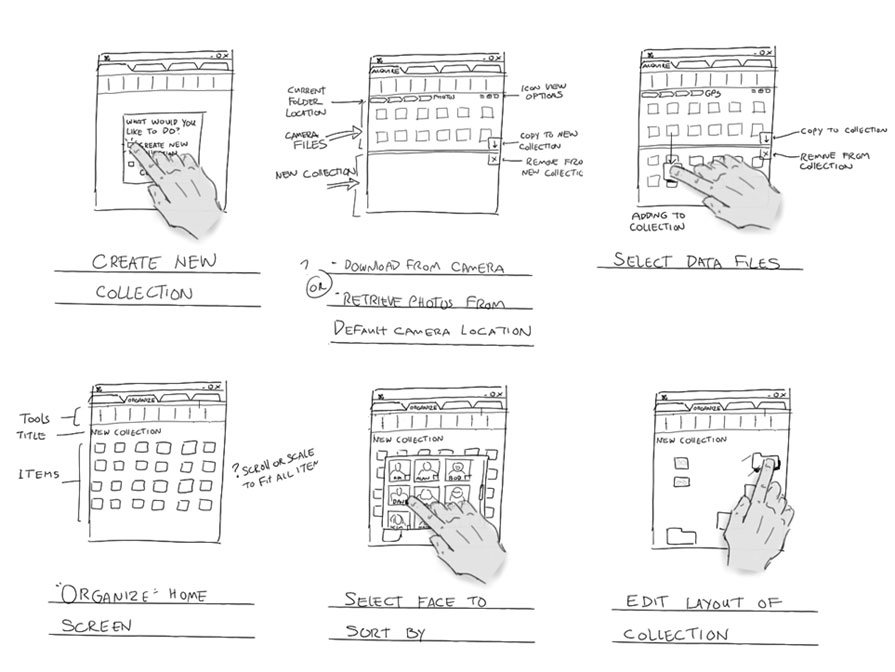
\includegraphics[keepaspectratio,width=\hsize,height=\halfh]
{images/storyboard.jpeg}

\caption[Storyboard Sketching]{
Example of storyboard sketching for drag and drop animation 
\citep{microsoftStoryboard}.
\imgcredit{Used with permission from Microsoft - Microsoft Copyrighted Content 
Guidelines}
}
\label{fig:storyboard}
\end{figure}
